\chapter{État de l'Art}
\label{chap:etat_art}

\section{Introduction}

Dans le contexte de l'Industrie 4.0, la maintenance prédictive s'affirme comme un levier essentiel pour améliorer la disponibilité des équipements et réduire les arrêts non planifiés. Elle prolonge la maintenance conditionnelle en exploitant l'analyse des données de fonctionnement — notamment les vibrations — et des méthodes d'intelligence artificielle pour détecter précocement les comportements anormaux.

Toutefois, le déploiement de solutions complètes reste difficile pour de nombreuses entreprises en raison des coûts, de la complexité d'intégration et de la dépendance à des infrastructures réseau.

Dans ce cadre, le paradigme TinyML — exécuter des modèles d'IA directement sur des microcontrôleurs — offre une alternative intéressante pour analyser au plus près de la machine, avec une faible latence, une meilleure confidentialité et des coûts contenus.

Ce chapitre présente les bases théoriques (terminologie, analyse vibratoire, IA pour la détection d'anomalies, TinyML) et se conclut par une revue critique de la littérature afin d'identifier les lacunes et positionner la suite du mémoire.

\section{L'évolution des stratégies de maintenance industrielle}

La maintenance industrielle a progressivement évolué du réactif vers l'anticipatif, à mesure que la terminologie s'est normalisée, que la mesure en service s'est diffusée et que l'analytique des données s'est imposée.

Le cadre de référence adopté dans ce mémoire est celui de la norme EN 13306 (version européenne), qui définit la maintenance comme l'ensemble d'actions techniques, administratives et de management destiné à maintenir ou rétablir un bien dans l'état lui permettant d'assurer la fonction requise, et distingue notamment les catégories corrective, préventive, conditionnelle et prédictive \cite{en13306}.

\subsection{Du réactif au prédictif : un continuum de pratiques}

\subsubsection{Maintenance corrective (run-to-failure)}
L'intervention est réalisée après la panne. Cette stratégie, encore utilisée pour des actifs peu critiques, reste exposée aux arrêts non planifiés et aux risques de dommages collatéraux. Les définitions et distinctions associées sont cadrées par EN 13306 \cite{en13306}.

\subsubsection{Maintenance préventive systématique (calendaire/usage)}
Les interventions sont planifiées en fonction du temps ou de l'usage. Elle réduit certains aléas mais peut conduire au sur-entretien lorsque les intervalles ne reflètent pas la dégradation réelle (terminologie et catégories selon EN 13306) \cite{en13306}.

\subsubsection{Maintenance conditionnelle (CBM, condition-based maintenance)}
Les décisions sont fondées sur des indicateurs d'état mesurés en service (p. ex. vibrations, température, analyses de lubrifiants). La norme ISO 17359 fournit les lignes directrices pour établir un programme de surveillance : objectifs, choix des variables, fréquence d'acquisition, critères d'alarme et revue périodique du dispositif \cite{iso17359}. Les revues de référence montrent que la CBM a structuré le diagnostic/prognostic des machines et ouvert la voie à l'analytique avancée \cite{jardine2006,lee2014,hector2024,achouch2022}.

\subsubsection{Maintenance prédictive (PdM)}
Elle exploite l'analyse de données (statistique, apprentissage automatique) pour anticiper l'apparition d'anomalies et optimiser la planification des interventions. Les ouvrages et revues de référence décrivent la PdM comme l'extension analytique de la CBM (capteurs → extraction de caractéristiques → modèles de diagnostic/prognostic), trajectoire amplifiée par l'IIoT et l'IA au sein d'Industrie 4.0 \cite{mobley2002,lee2014,lasi2014,kagermann2013,hector2024,achouch2022}.

\begin{figure}[h]
\centering
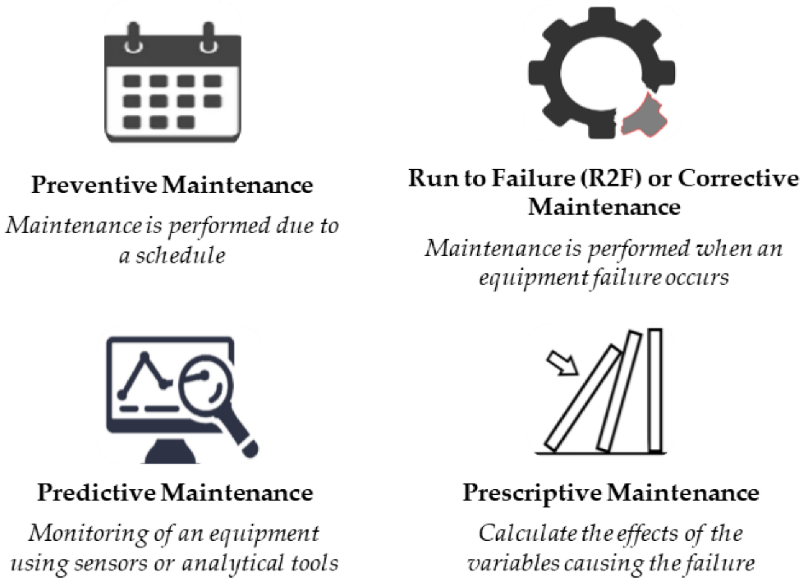
\includegraphics[width=0.85\textwidth]{images/maintaince-types.png}
\caption{Typologie des stratégies de maintenance.}
\label{fig:maintenance_types}
\end{figure}

\subsection{Enjeux économiques et opérationnels}

Les arrêts non planifiés constituent un poste majeur de pertes dans l'industrie, d'où l'intérêt de stratégies fondées sur les données pour améliorer la disponibilité et la planification des interventions.

Des analyses industrielles rapportent que, selon les contextes, la maintenance prédictive peut réduire le temps d'arrêt de 30 à 50 \% et prolonger la durée de vie des actifs de 20 à 40 \% (ordre de grandeur consolidé par McKinsey \cite{mckinsey2017}). Ces bénéfices restent dépendants de la qualité de mise en œuvre (gestion des faux positifs, gouvernance des données) \cite{mckinsey2021}.

Par ailleurs, des études sectorielles mettent en évidence le coût élevé d'une heure d'arrêt (ordre de grandeur fourni par le rapport industriel Siemens/Senseye 2024) \cite{siemens2024}, ce qui motive des approches au plus près de la machine mieux maîtrisée localement.

Enfin, pour les PME, des obstacles récurrents (compétences, capital, infrastructures, cybersécurité) freinent l'adoption de solutions lourdes et justifient des alternatives edge/TinyML plus frugales \cite{oecd2021}.

\subsection{Facteurs récents d'évolution}

Trois leviers structurent la diffusion des approches conditionnelles et prédictives :

\begin{enumerate}
\item \textbf{Normalisation et bonnes pratiques.} EN 13306 fournit une terminologie partagée de la maintenance, ISO 17359 décrit le déploiement opérationnel d'un programme de surveillance d'état (objectifs, variables, fréquence, critères d'alarme, revue) \cite{en13306,iso17359}.

\item \textbf{Instrumentation et données.} La généralisation des capteurs (p. ex. vibration) et des systèmes d'acquisition a permis de passer du seuil aux modèles de diagnostic/prognostic, comme l'attestent les revues CBM/PdM \cite{jardine2006,lee2014,hector2024,achouch2022}.

\item \textbf{Numérisation (Industrie 4.0) et Edge.} L'IIoT connecte les actifs, tandis que l'edge computing rapproche l'analyse de la machine (latence réduite, trafic moindre, meilleure confidentialité), préparant l'embarqué (TinyML) détaillé plus loin \cite{lasi2014,kagermann2013,shi2016,kong2022}.
\end{enumerate}

\subsection{Pont vers l'analyse vibratoire (normes applicables)}

Pour les machines tournantes, la surveillance vibratoire constitue une modalité majeure d'observation. L'évaluation de la sévérité vibratoire s'appuie sur ISO 20816-1, qui établit les conditions générales de mesure et d'évaluation des vibrations de machines (successeur de la série 10816) \cite{iso20816-1}. Cette référence normative sera mobilisée pour situer les niveaux et indicateurs pertinents avant d'aborder l'analyse fréquentielle (FFT) et les signatures de défaut, voir ISO 10816-3 pour des cas d'usage industriels courants \cite{iso20816-3}.

Des ressources récentes synthétisent les principes et pratiques de l'analyse vibratoire pour la maintenance conditionnelle (tutoriel et panorama capteurs) \cite{matania2024,hassan2024}, en complément des revues et manuels de référence \cite{tiboni2022,mobley2002}.

\begin{table}[ht]
\centering
\caption{Panorama des stratégies de maintenance (Sources : EN 13306 \cite{en13306}, ISO 17359 \cite{iso17359}, Jardine \cite{jardine2006}, Lee \cite{lee2014}, Mobley \cite{mobley2002}).}
\label{tab:maintenance_strategies}
\small
\begin{tabular}{p{2.2cm}p{3.3cm}p{3.8cm}p{3.8cm}}
\toprule
\textbf{Paradigme} & \textbf{Déclencheur d'intervention} & \textbf{Atouts} & \textbf{Limites} \\
\midrule
Corrective & Panne avérée & Simplicité de planification & Arrêts non planifiés, risques collatéraux \\
Préventive (calendaire/ usage) & Échéance/ compteur & Réduction d'aléas connus & Sur-entretien possible \\
Conditionnelle (CBM) & Indicateurs d'état mesurés & Intervention ciblée, suivi d'état & Instrumentation et processus à structurer \\
Prédictive (PdM) & Modèles diagnostic/ prognostic & Anticipation, optimisation décision & Exigences données et compétences \\
\bottomrule
\end{tabular}
\end{table}

\section{Concepts fondamentaux}

\subsection{Stratégies de surveillance d'état}

La maintenance conditionnelle s'appuie sur différentes modalités de mesure (surveillance d'état) dont le choix dépend des mécanismes de défaillance, du coût et des contraintes d'exploitation. Les lignes directrices pour établir un programme de condition monitoring sont décrites par ISO 17359 (objectifs, variables, fréquence, critères d'alarme) \cite{iso17359}.

Les revues confirment l'usage des modalités suivantes dans l'industrie et la recherche récente \cite{tiboni2022,hector2024,achouch2022} :

\begin{itemize}
\item \textbf{Vibration (accélération/vitesse/déplacement)} : sensible aux défauts mécaniques des machines tournantes (balourd, désalignement, roulements), riche en information et fortement normalisée pour l'évaluation (ISO 20816-1 / 10816-3) \cite{iso20816-1,iso20816-3,tiboni2022,matania2024}.

\item \textbf{Analyse d'huile / débris} : usure et contamination (métaux, particules), utile pour réducteurs/roulements mais nécessite prélèvements/analyses spécifiques \cite{iso17359,hector2024}.

\item \textbf{Thermographie / température} : utile pour frottements, défauts d'isolation ou surcharge, moins spécifique à certains défauts mécaniques \cite{iso17359,hector2024}.

\item \textbf{Acoustique / émissions acoustiques} : sensible aux chocs/naissances de fissures, instrumentation et interprétation plus délicates \cite{tiboni2022,hector2024}.

\item \textbf{Signaux électriques (MCSA, courant/tension)} : utile pour défauts moteurs (barres de rotor, excentricité), moins direct pour la chaîne mécanique aval \cite{hector2024,achouch2022}.
\end{itemize}

\textbf{Pourquoi la vibration dans notre contexte :} (i) Couverture de défauts mécaniques dominants des machines tournantes (signatures bien établies), (ii) capteurs MEMS abordables et faciles à intégrer, (iii) cadres normatifs clairs pour la mesure/évaluation, (iv) chaînes de traitement compatibles MCU (FFT + indicateurs) \cite{iso20816-1,iso20816-3,tiboni2022,matania2024}.

\subsection{Signatures vibratoires des défauts}

Dans les machines tournantes, des motifs fréquentiels récurrents guident le diagnostic :

\begin{itemize}
\item \textbf{Balourd} : pic dominant à 1×fr (parfois faibles harmoniques)
\item \textbf{Désalignement} : harmoniques marquées (2×, 3×)
\item \textbf{Roulements} : pics aux fréquences caractéristiques (BPFO/BPFI/BSF/FTF) et bandes latérales
\item \textbf{Jeu / défauts structuraux} : énergie large bande accrue
\end{itemize}

Ces motifs sont synthétisés dans des tutoriels et revues récentes \cite{tiboni2022,matania2024} et s'interprètent dans le cadre d'ISO 20816-1 / 10816-3 pour situer la sévérité \cite{iso20816-1,iso20816-3}.

Les formules (FTF, BPFO, BPFI, BSF) et les rappels FFT / résolution spectrale figurent en Annexe avec les sources de référence \cite{bkvibro2002,randall2011,oppenheim2010,cooley1965}.

\subsection{Apprentissage automatique (ML)}

Par apprentissage automatique (ML), on désigne des méthodes apprenant des structures à partir des données pour assister le diagnostic/prognostic en maintenance \cite{jardine2006,lee2014}.

On distingue classiquement :

\begin{itemize}
\item \textbf{Supervisé (étiquettes disponibles)} : classification/régression (SVM, RF, CNN/LSTM 1-D sur signaux/spectres) — bonnes performances si des données étiquetées de qualité existent \cite{lee2014,achouch2022}.

\item \textbf{Non-supervisé (peu/pas d'étiquettes)} : détection d'anomalies par seuillage/statistique, clustering (p. ex. K-means, DBSCAN), frontière (One-Class SVM) ou reconstruction (autoencoders). Ces approches apprennent la normalité et signalent les écarts \cite{chandola2009,hector2024,achouch2022,macqueen1967}.
\end{itemize}

\subsection{Edge AI et TinyML}

L'Edge AI exécute le traitement au plus près de la machine, réduisant latence et trafic et améliorant la confidentialité par rapport au cloud \cite{shi2016,kong2022}.

Le TinyML cible les microcontrôleurs (RAM/Flash/puissance limitées) via des optimisations (quantification, élagage) et des modèles compacts \cite{warden2019,reddi2022,tsoukas2024}.

\textbf{Runtime et benchmarks} : TensorFlow Lite Micro (TFLM) fournit un runtime C/C++ sans OS adapté MCU (opérateurs sélectionnés, mémoire statique) \cite{david2021}. MLPerf Tiny propose des benchmarks pour comparer précision/latence/consommation en contexte edge \cite{banbury2021}.